\section{Strukturmuster}
\label{sec:Kap-10.2}

\textit{Strukturmuster} beschreiben, wie Klassen bzw. ihre Instanzen zu größeren Strukturen zusammengesetzt werden können. In \cite{gam95} finden wir folgende sieben Strukturmuster:

\begin{description}
	\setlength{\itemsep}{2mm} %%% für Druck
	
	\item[\textit{Adapter}] (adapter) wandelt die Schnittstelle (gegebener) dienstleistender Klassen so um, dass dienstnutzende Klassen sie verwenden können.
	\item[\textit{Brücke}] (bridge) entkoppelt eine Abstraktion von ihrer Implementierung, damit beide unabhängig voneinander verändert werden können.
	\item[\textit{Dekorateur}] (decorator) heftet dynamisch zusätzliche Verantwortlichkeiten (Operationen) an ein Objekt. Dekorateure basieren auf Dienstnutzungen und stellen für die Funktionalitätserweiterung eine flexible Alternative zur Generalisierung dar.
	\item[\textit{Fassade}] (facade) stellt eine einheitliche Schnittstelle für eine Menge von Schnitt\-stellen zur Verfügung und führt eine Strukturierungsebene oberhalb von Klassen ein.
	\item[\textit{Fliegengewicht}] (flyweight) benutzt wenige (komplexe) Objekte mehrfach (shared objects), um eine große Anzahl kleiner Objekte effizient handhaben zu können.
	\item[\textit{Kompositum}] (composite) ermöglicht den einheitlichen Zugriff auf die Elemente hierarchisch strukturierter Objektstrukturen und bietet dafür eine Schnittstelle, mit der individuelle Objekte (Blätter eines Baums) und Kompositionen (innere Knoten) gleichbehandelt werden können.
	\item[\textit{Proxy}] (proxy) stellt über ein stellvertretendes Objekt eingeschränkte Zugriffe auf das eigentliche Objekt zur Verfügung.
\end{description}

\vspace{\baselineskip} %%% für Druck

\vspace{\baselineskip}
\textcolor{FernUni-MI-green}{\noindent\rule[1ex]{\textwidth}{2pt}}\\
{\Large \textcolor{FernUni-MI-green}{\textsc{Fassade}}}\\
\textcolor{FernUni-MI-green}{\noindent\rule[1ex]{\textwidth}{2pt}}

\begin{description}
	\setlength{\itemsep}{2mm} %%% für Druck
	
	\item[Zweck] Stellt eine einheitliche Schnittstelle für eine Menge von Schnittstellen zur Verfügung und führt eine Strukturierungsebene oberhalb von Klassen ein.
	\item[Motivation] Ein häufiges Ziel im Entwurf ist die Minimierung der Abhängigkeiten zu einer Gruppe von eng zusammenarbeitenden Klassen (einem Cluster). Ein Weg zur Erreichung dieses Zieles ist der Einsatz eines Fassaden-Objekts, welches eine einfache Schnittstelle zu der Funktionalität des Clusters anbietet (Abb.~\ref{fig:muster_fassade}).
	
\clearpage %%% für Druck

\vspace*{2mm} %%% für Druck

	\begin{figure}[h!]
		\centering
		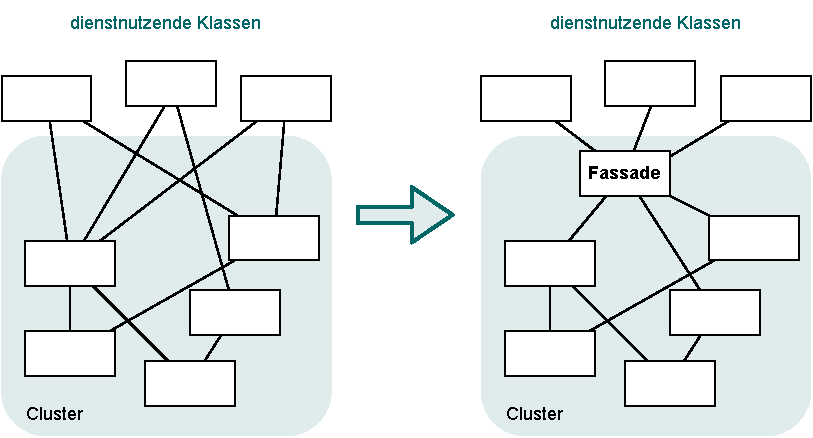
\includegraphics{Bilder/Kapitel-10/muster_fassade.pdf}
		\caption{Grundstruktur des Fassade-Musters}
		\label{fig:muster_fassade}
	\end{figure}

	\item[Anwendbarkeit] Man verwendet das Muster Fassade unter folgenden Bedingungen:
	\begin{itemize}
		\item 	Ein komplexes Cluster soll eine einfache Schnittstelle erhalten. Cluster werden häufig im Lauf ihrer Entwicklung komplexer. Die meisten Muster führen durch ihre Anwendung zu mehr und kleineren Klassen. Die Anwendung des Musters Fassade macht die Cluster besser wiederverwendbar und adaptierbar, gleichzeitig wird ihre Nutzung aber für jene schwieriger, die keine Adaptierung für ihre Aufgabenstellung benötigen. Eine Fassade bietet eine einfache Standardsicht des Clusters an, die für die meisten Dienstnutzer ausreicht.
		\item 	Es existieren viele Abhängigkeiten zwischen den Dienstnutzern und den Implementierungsklassen einer Abstraktion. Man verwendet das Muster Fassade, um die Abhängigkeiten zwischen den Dienstnutzern und dem Cluster in der Fassaden-Klasse zu konzentrieren und dadurch seine Unabhängigkeit und Portabilität zu erhöhen.
		\item 	Dienstnutzer, die eine größere Flexibilität oder umfangreichere Funktionalität benötigen, müssen unter Umgehung der Fassade auf einzelne Klassen des Clusters zurückgreifen.
	\end{itemize}
	
	\item[Zusammenspiel] Dienstnutzer kommunizieren mit dem Cluster, indem sie Methoden der Fassade aufrufen, welche die Aufrufe an die entsprechenden Objekte des Clusters weiterleiten. Obwohl die Clusterobjekte die eigentliche Arbeit leisten, muss die Fassade eventuell selbst Arbeit leisten, um ihre Schnittstelle in die Schnittstellen der Clusterobjekte zu übersetzen. Die Dienstnutzer der Fassade können auf alle oder ausgewählte Objekte des Clusters direkt zugreifen, indem sie vom Fassadenobjekt eine Referenz auf diese Objekte anfordern.
	\item[Konsequenzen] Das Muster Fassade hat folgende Vorteile:
	\begin{itemize}
		\item 	Es trennt Dienstnutzer von Objekten eines Clusters und reduziert dadurch die Anzahl der Objekte, mit denen der Dienstnutzer zu tun hat. Dadurch wird die Benutzung des Clusters einfacher.
		\item 	Es reduziert die Kopplung zwischen dem Dienstnutzer und den Objekten eines Clusters.
		\item 	Es verhindert nicht die direkte Nutzung der Objekte des Clusters durch Anwendungen, falls dies notwendig ist. Man kann zwischen einer ein\-fachen Benutzung und vollständigem Funktionsumfang wählen.
	\end{itemize}

	\item[Implementierung] Eine Möglichkeit die Kopplung zwischen Dienstnutzern und \linebreak %%% für Druck
	Cluster weiter zu reduzieren, ist die Realisierung der Klasse Fassade als abstrakte Klasse oder Interface. So ist der Dienstnutzer nicht an eine konkrete Implementierung eines Clusters gebunden.
	
	Ein Cluster kann in Java als Paket realisiert werden, wobei die Fassaden-Klasse und ausgewählte Klassen des Clusters außerhalb des Paketes sichtbar sind, alle anderen Klassen des Clusters aber nur innerhalb des Pakets.	
\end{description}